\documentclass[10pt]{article}
\usepackage{hyperref}
\usepackage[utf8]{inputenc}
\usepackage[swedish]{babel}
\usepackage[margin=2cm]{geometry}
\usepackage{calc}
\usepackage{graphicx}
\usepackage{filecontents}
\usepackage{etoolbox}
\usepackage{enumitem}
\usepackage[backend=bibtex,sorting=none,style=numeric,natbib=true]{biblatex}
\graphicspath{ {images/}}

\selectlanguage{swedish}

\tolerance=1
\emergencystretch=\maxdimen
\hyphenpenalty=10000
\hbadness=10000

% Variable för att räkna ut magnituden på en risk.
\newcounter{indexcounter}
% Macros för risker, för att strukturera upp dem.
\newcommand{\Krav}[2]{
	\stepcounter{indexcounter}
	Krav \arabic{indexcounter} & #1 & #2 \\ \hline
}
\newcommand{\History}[3]{
	\centering #1 & #2 & #3 \\ \hline
}

\addbibresource{kravspecifikation.bib}

\title{Kravspecifikation}

\author{
    Joel Almqvist\\
    \texttt{joeal360@student.liu.se}
    \and
    Björn Detterfelt\\
    \texttt{bjode786@student.liu.se}
    \and
    Tim Håkansson\\
    \texttt{timha404@student.liu.se}
    \and
    David Kjellström\\
    \texttt{davkj168@student.liu.se}
    \and
    Axel Löjdquist\\
    \texttt{axelo225@student.liu.se}
    \and
    Joel Oskarsson\\
    \texttt{joeos014@student.liu.se}
    \and
    Lieth Wahid\\
    \texttt{liewa893@student.liu.se}
    \and
    Alexander Wilkens\\ 
    \texttt{alewi684@student.liu.se}
}

\date{\today \\Version 2.0}

\begin{document}

\maketitle
\pagebreak

\section*{Dokumenthistorik}

\begin{center}
    \begin{tabular}{|p{1.5cm}|p{2cm}|p{12cm}|}
    	\hline
        \textbf{Version} & \textbf{Datum} & \textbf{Förändring och kommentar} \\ \hline
        \History{1.0}{2018-02-15}{Första utkast till kund}
        \History{1.1}{2018-02-16}{Uppdaterat stavning, definitioner, formulerat om krav 3, 9, 11, 16, 22 ,23 \& 24. Tog bort krav 12, 13, 17, 19, 20 \& 21. (Kund)}
        \History{1.2}{2018-02-19}{Uppdaterat stavning, formulerat om krav 8 \& 16. (Kund)}
        \History{1.3}{2018-02-22}{Uppdaterat stavning, formulerat om krav 6, 8, 10, 13, 15, 17, 22, 23, 28 \& 32. (Kund)}
        \History{1.4}{2018-02-27}{Uppdaterat stavning och struktur. Lagt till en översiktlig bild av systemet. Formulerat om krav 17, 24, 33  \& 34. (Handledare)}
    \end{tabular}
\end{center}

\pagebreak
\tableofcontents
\pagebreak

\section{Inledning}
	I detta kapitel definieras och introduceras kontexten för projektet som ska utföras.

	\subsection{Definitioner}
		\begin{itemize}[leftmargin=5cm]
		\item [UI-applikationen] Applikationen som tar emot kontrolldata och använder denna data för att sköta spellogik och grafik.
		\item [Kontrollapplikationen] Applikationen som körs på en mobil eller surfplatta som styr spelet
		\item [Sensor] En apparat eller anläggning som insamlar data. Vi syftar ej på en touch-skärm när vi refererar till en sensor.
		\item [Spelinstans] Ett spel med en unik identifikationskod
		\item [PWA (Progressive Web App)] Ett mellanting mellan en hemsida och en applikation. En PWA är en vanlig hemsida som beter sig som en app.
		\item [Realtidsmultiplayerspel] Spel där flera användares handlingar har en direkt inverkan på spelets tillstånd.
		\item [Gamemode] En variant av basspelet med eventuellt andra funktioner och regler.
		\item [Vanliga nätverksförhållanden] En enhet med en stabil internetuppkoppling utan yttre störningar.
		\end{itemize}	

	\subsection{Parter}
	Kunden till projektet är Cybercom Sweden. Projektet utförs av projektgruppens medlemmar.
	
	\subsection{Syfte \& mål}
	Syftet med detta dokument är att förtydliga vad som förväntas vara klart vid projektets slut. Dokumentet fungerar som överenskommelse mellan kunden Cybercom Sweden och projektgruppen. Kraven specificerar vilken funktionallitet, kvalitet och design produkten ska uppfylla. Dokumentet utgör grunden för hur hela projektet ska struktureras och utformas. Kraven är framtagna efter Cybercom Swedens önskemål och formulerade för att ligga till stöd för projektgruppensarbete.
	
	\subsection{Användning}
		För att kunna använda produkten måste två olika applikationer köras på minst två olika enheter. En mobil eller surfplatta ska användas som kontroll för att styra spelet och kommer att köra kontrollapplikationen. Utöver detta ska en enhet som t.ex. en dator vara uppkopplad till en skärm. Datorn ska köra själva spelet och kommer att köra UI-applikationen. Se \ref{fig:overview} för en översiktlig bild av systemet. \\
\\
För att kunna använda produkten startar man UI-applikationen. Då UI-applikationen körs igång, skapas en spelinstans där en identifikationskod kommer att genereras och visas på skärmen. För att kunna ansluta sig till den spelinstansen behöver en användare starta kontrollapplikationen. Här kommer användaren behöva ange ett användarnamn samt identifikationskoden. Efter att användaren har gjort detta, är spelet redo att spelas.

\pagebreak

\section{Översikt av Systemet}
	Detta kapitel ger en överskådlig blick av systemet.
	
	\begin{figure}[h]
		\centering
		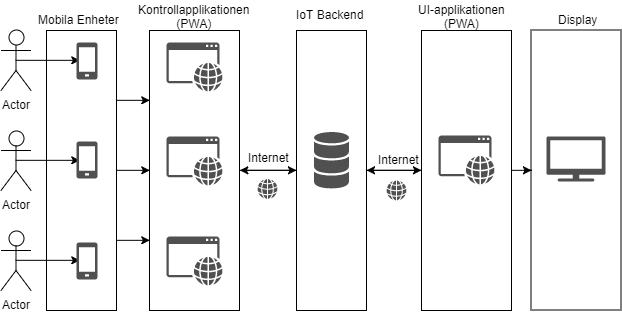
\includegraphics[scale=0.8]{overview}
		\caption{Översikt av systemet}
		\label{fig:overview}
	\end{figure}

	\subsection{Grov beskrivning av produkten}
	Produkten ska vara ett realtidsmultiplayerspel. Spelet är uppdelat i två olika applikationer, en UI-applikation och en kontrollapplikation. Det är tänkt att UI-applikationen ska agera skärm för spelet och kan liknas med en konsol för ett TV-spel. På denna del kommer själva spelet köras och vara uppkopplad till en skärm där spelet visas. En kontroller kommer vara antingen en mobil eller surfplatta och kan liknas med spelkontrollerna till konsolen. Enhetens sensorer används för att spelaren ska kunna styra spelet. Kommunikationen mellan UI-applikationen och kontrollapplikationen kommer att ske genom Cybercoms IoT-backend, se \ref{fig:backend}. Att kommunikationen går genom Cybercoms IoT-backend är vitalt eftersom huvudsyftet med projektet är att demonstrera Cybercoms IoT-backend.  Både kontroll- och UI-Applikationen kommer att utvecklas som PWA:s. 
	
	\begin{figure}[h]
		\centering
		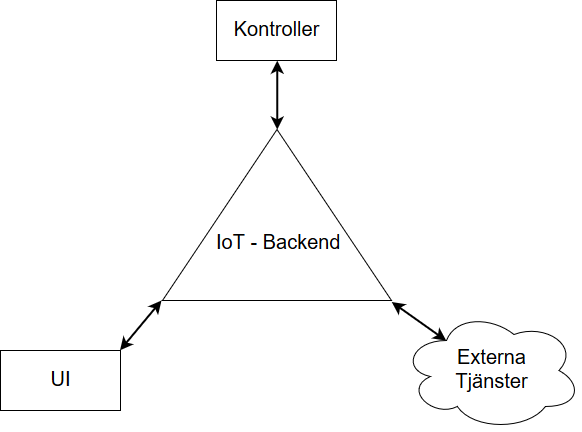
\includegraphics[scale=0.4]{backend}
		\caption{Kommunikation mellan Cybercoms IoT-backend och komponenterna i systemet}
		\label{fig:backend}
	\end{figure}
	
	
	\subsection{Beroenden av andra system}
	Produkten är beroende av Cybercoms IoT-backend då all kommunikation måste gå genom denna. Både kontroll- och UI-applikationen är beroende av en enhet som har tillgång till version 64 av Google Chrome. En enhet kan t.ex. vara en dator, surfplatta eller en mobil. Enheten måste ha en internetanslutning.

\pagebreak
\section{Krav}
	Detta avsnitt listar alla krav som sätts på produkten. Krav med prioritet 1 förväntas vara avklarade vid projektetsslut. Krav med prioritet 2 ska arbetas mot då alla krav med prioritet 1 är avklarade. Kraven är uppdelade i följande kategorier: funktionella krav och design- och kvalitetskrav. Varje krav består av ett unikt nummer, en beskrivning samt en prioritet.
	
	\subsection{Funktionella Krav}
	Detta avsnitt listar de funktionella kraven på produkten. Funktionella krav deklarerar vilka beteenden och attribut produkten förväntas ha. 

	\subsubsection*{Generella krav}
	Nedan följer generella krav för både kontroll- och UI-applikationen.\\
	
	\begin{tabular}{| p{2cm} | p{8cm} | p{2cm}|}
		\hline
		
		\textbf{Krav nr.} & \textbf{Beskrivning} &\textbf{Prioritet} \\ \hline
		\Krav{En mobil eller surfplatta ska användas som spelkontroll för spelet.}{1}
		\Krav{UI-applikationen ska endast kommunicera med \newline kontrollapplikationen via  Cybercoms IoT-backend.}{1}
		\Krav{En användare ska kunna ansluta sig till en spelinstans.}{1}
		\Krav{Flera instanser av spelet ska kunna köras samtidigt.}{1}
		\Krav{En unik slumpmässig identifikationskod ska genereras för en spelinstans.}{1}
		\Krav{Spelet ska stödja flera gamemodes.}{2}
		\Krav{En spelare ska ha möjligheten att rösta på vilket gamemode som ska spelas.}{2}
				
	\end{tabular}

	\subsubsection*{Krav kontrollapplikation}
	Nedan följer krav specifika för kontrollapplikationen.\\

	\begin{tabular}{| p{2cm} | p{8cm} | p{2cm}|}
		\hline
		
		\textbf{Krav nr.} & \textbf{Beskrivning} &\textbf{Prioritet} \\ \hline
		\Krav{Kontrollapplikationen ska ha ett grafiskt gränssnitt.}{1}
		\Krav{Spelaren ska kunna sätta ett användarnamn.}{1}
		\Krav{Om en spelare inte anger ett användarnamn, ska ett användarnamn ges till spelaren.}{1}
		\Krav{Kontrollapplikationen ska köras på en enhet som har minst version 64 av Google Chrome.}{1}
		\Krav{Kontrollapplikationen ska ansluta sig till en spelinstans genom att välja en spelinstans från en lista.}{1}
		\Krav{Kontrollapplikationen ska ha en sökruta, för att kunna söka bland de olika spelinstanserna.}{1}
		\Krav{Kontrollapplikationen ska kommunicera med Cybercoms IoT-backend.}{1}
		\Krav{Kontrollapplikationen ska kunna kalibrera en accelerometer.}{1}
		\Krav{Kontrollapplikationen ska stödja alternativa styrningsmetoder i de fall sensorer saknas.}{2}
		\Krav{Kontrollapplikationen ska stödja styrning med tangentbord och mus.}{2}

	\end{tabular}

	\pagebreak
	\subsubsection*{Krav UI-applikation}
	Nedan följer krav specifika för UI-applikationen.\\

	\begin{tabular}{| p{2cm} | p{8cm} | p{2cm}|}
		\hline
		
		\textbf{Krav nr.} & \textbf{Beskrivning} &\textbf{Prioritet} \\ \hline
		\Krav{UI-applikationen ska stödja minst fem spelare samtidigt.}{1}
		\Krav{UI-applikationen ska ha ett grafiskt gränssnitt.}{1}
		\Krav{UI-applikationen ska kunna köras på en enhet som har minst version 64 av Google Chrome.}{1}
		\Krav{UI-applikationen ska kommunicera med Cybercoms IoT-backend.}{1}
		\Krav{UI-applikationen ska visa en unik kod för sin spelinstans.}{1}
		\Krav{UI-applikationen ska arkitekturellt ha stöd för godtyckligt antal spelare. Hårdvara, prestanda och plats på skärmen begränsar.}{2}
		\Krav{UI-applikationen ska kunna visa det som andra UI-applikationer visar i realtid.}{2}
						
	\end{tabular}
	
	\subsection{Designkrav}
	Detta avsnitt listar designkraven på produkten. Designkrav specificerar hur produkten ska utformas och ställer krav på hur utvecklingsprocessen kommer gå tillväga.  \\
	
	\begin{tabular}{| p{2cm} | p{8cm} | p{2cm}|}
		\hline
		\textbf{Krav nr.} & \textbf{Beskrivning} & \textbf{Prioritet} \\ \hline
		
		\Krav{UI-applikationen ska skrivas i Javascript ES2015+.}{1}
		\Krav{Kontrollapplikationen ska skrivas i Javascript ES2015+.}{1}
		\Krav{UI-applikationen ska utvecklas som en PWA.}{1}
		\Krav{Kontrollapplikationen ska utvecklas som en PWA.}{1}
		\Krav{UI-applikationen ska licensieras under MITs open source licens.}{1}
		\Krav{Kontrollapplikationen ska licensieras under MITs open source licens.}{1}
		\Krav{Applikationsprojekten ska vara Node-baserade.}{1}
		
	\end{tabular}
\pagebreak
	\subsection{Kvalitetskrav}
	Detta avsnitt listar kvalitetskraven på produkten. Kvalitetskrav specificerar hur väl ett attribut hos produkten måste funktionera. D.v.s. vilka kvaliteer en lösning måste ha eller under vilka förhållanden lösningen måste fungera inom.  \\
	
		\begin{tabular}{|p{2cm}|p{8cm}|p{2cm}|}
		\hline
		\textbf{Krav nr.} & \textbf{Beskrivning} & \textbf{Prioritet} \\ \hline
		
		\Krav{UI-applikationen ska kunna köras i 4 timmar utan avbrott.}{1}
		\Krav{Koden ska följa en enhetlig standard\cite{bib-kvalitetsplan} för att underlätta vidareutveckling av projektet.}{1}
		\Krav{Tiden att ansluta sig till en spelsession får inte överskrida 10 sekunder under vanliga nätverksförhållanden.}{1}
        \Krav{Enkätens\cite{bib-kvalitetsplan} genomsnittliga betyg för responsivitet ska åtminstone vara 6 av 10 vid en undersökning av 20 deltagare.}{1}
		\Krav{Enkätens\cite{bib-kvalitetsplan} genomsnittliga betyg för användbarhet ska åtminstone vara 6 av 10 vid en undersökning av 20 deltagare.}{1}
		\Krav{Enkätens\cite{bib-kvalitetsplan} genomsnittliga betyg för den alternativa styrningen ska åtminstone vara 6 av 10 vid en undersökning av 20 deltagare.}{1}
		\Krav{Enkätens\cite{bib-kvalitetsplan} genomsnittliga betyg för ''lätt att förstå vad som händer'' ska åtminstone vara 6 av 10 vid en undersökning av 20 deltagare.}{1}
				
	\end{tabular}
	

\pagebreak

\printbibliography
\addcontentsline{toc}{section}{\refname}


\end{document}
